% CVPR 2022 Paper Template
% based on the CVPR template provided by Ming-Ming Cheng (https://github.com/MCG-NKU/CVPR_Template)
% modified and extended by Stefan Roth (stefan.roth@NOSPAMtu-darmstadt.de)

\documentclass[10pt,twocolumn,letterpaper]{article}

%%%%%%%%% PAPER TYPE  - PLEASE UPDATE FOR FINAL VERSION
%\usepackage[review]{cvpr}      % To produce the REVIEW version
\usepackage{cvpr}              % To produce the CAMERA-READY version
%\usepackage[pagenumbers]{cvpr} % To force page numbers, e.g. for an arXiv version

% Include other packages here, before hyperref.
\usepackage{graphicx}
\usepackage{amsmath}
\usepackage{amssymb}
\usepackage{booktabs}

\usepackage{makecell}
\usepackage{mathtools}

% It is strongly recommended to use hyperref, especially for the review version.
% hyperref with option pagebackref eases the reviewers' job.
% Please disable hyperref *only* if you encounter grave issues, e.g. with the
% file validation for the camera-ready version.
%
% If you comment hyperref and then uncomment it, you should delete
% ReviewTempalte.aux before re-running LaTeX.
% (Or just hit 'q' on the first LaTeX run, let it finish, and you
%  should be clear).
\usepackage[pagebackref,breaklinks,colorlinks]{hyperref}


% Support for easy cross-referencing
\usepackage[capitalize]{cleveref}
\crefname{section}{Sec.}{Secs.}
\Crefname{section}{Section}{Sections}
\Crefname{table}{Table}{Tables}
\crefname{table}{Tab.}{Tabs.}


%%%%%%%%% PAPER ID  - PLEASE UPDATE
\def\cvprPaperID{*****} % *** Enter the CVPR Paper ID here
\def\confName{CVPR}
\def\confYear{2022}


\begin{document}

%%%%%%%%% TITLE - PLEASE UPDATE
\title{Spectrogram Augmentation Using Image Processing Techniques}

\author{Hejung Yang\\
Yonsei University\\
{\tt\small hejung.yang@dsp.yonsei.ac.kr}
}
\maketitle

%%%%%%%%% ABSTRACT
\begin{abstract}
   In speech processing, many data augmentation schemes exist regarding spectrogram as an image.
   These spectrogram augmentation plays an important role in improving performance, preventing 
   overfitting and making up for sparsity of the existing clean dataset.
   In this paper, various image processing techniques are applied for several speech processing tasks.
   Specifically, both spatial-domain and frequency-domain filtering ideas from image processing domain 
   are utilized. Additionally, commonly used image augmentation techniques are tested on the speech 
   processing task. In order to see the flexibilities on importing image augmentation methodologies onto speech,
   both speaker identification and speaker verification tasks are considered as the target in the experiments.
   It could be seen that all of the techniques could introduce either performance gain or task-specific 
   advantages, which increases anticipation on further applying augmentation ideas from image processing domain to 
   the speech domain.
\end{abstract}

%%%%%%%%% BODY TEXT
\section{Introduction}
\label{sec:intro}

In most supervised training of the deep neural network, the amount of training data heavily affects
the model quality in real-world test sets. However, in many cases, there exists not enough amount of 
training data to get the satisfied results. Given sparse training set, the model tends to overfit with low 
generalization power, resulting low performance in evaluation.
To mitigate the problem, various data augmentation schemes arose. 

In speech processing related tasks, both time-domain, frequency-domain related augmentation methods
are largely used to supplement the lack of dataset. Warping on either time or frequency axis is suggested 
from ~\cite{jaitly2013vocal}, ~\cite{ko2015audio}. ~\cite{salamon2017deep} includes pitch shifting, 
dynamic range compression for further augmentation. 
When converting 1-dimensional signal into spectrogram by applying Short-Time Fourier Transorm and 
interpreting the signal as a mixture of temporal-frequency
components, it is also possible to view the signal as an image. 
Some of the recent augmentation schemes perform augmentation base on the spectrogram, including 
SpecAugment~\cite{park2019specaugment} and SpecAugment++~\cite{wang2021specaugment++}.

This paper shows several spectrogram based augmentation schemes conducted with the help of image processing techniques,
especially in spatial filter and notch filter. Furthermore, commonly used image augmentation methodologies
are tested on speech processing domain.

\section{Augmentation schemes}
\subsection{spatial filter on spectrogram}
\label{sec:spatial}

Joint bilateral filter~(\cite{eisemann2004flash}, ~\cite{petschnigg2004digital}) is a variation of the 
bilateral filter first introduced to preserve precise edge components from the high-resolution depth 
image while smoothing out noisy artifacts.

Given input image $I$, reference image $J$ with smoothing parameters $\sigma_s$, $\sigma_r$,
joint bilateral smoothing works as follows:
\begin{equation}
\begin{multlined}
JointBilateral(p, I, J, \sigma_s, \sigma_r) = \\
1/K_p\sum_{q \in N(p)}exp(-\frac{||p-q||^2}{2\sigma_s^2}-\frac{||J(p)-J(q)||^2}{2\sigma_r^2})I(q)
\end{multlined}
\end{equation}
\begin{equation}
K_p = \sum_{q \in N(p)}exp(-\frac{||p-q||^2}{2\sigma_s^2}-\frac{||J(p)-J(q)||^2}{2\sigma_r^2})
\end{equation}
where $N(p)$ stands for the set of neighboring pixels of $p$.

From the fact that joint bilateral filter utilizes reference 
image for better noise suppression, in case where both the original and noisy image are given, it is expected
that the filter would generate the image which is almost identical to the original with appropriate adjustment 
of the parameters $sigma_s$ and $sigma_r$.
However, as the nature of the bilateral filter is to "smooth out" the image, 
while it seems that the noisy components are completely removed,
it is rather embedded all over the image. Thus it can be expected that the denoised image contains both the 
characteristics of the original image and the inherent noisy pattern. From this hypothesis, denoised spectrogram
using the bilateral filter is used for training speech processing model.

\begin{figure*}[h]
   \centering
   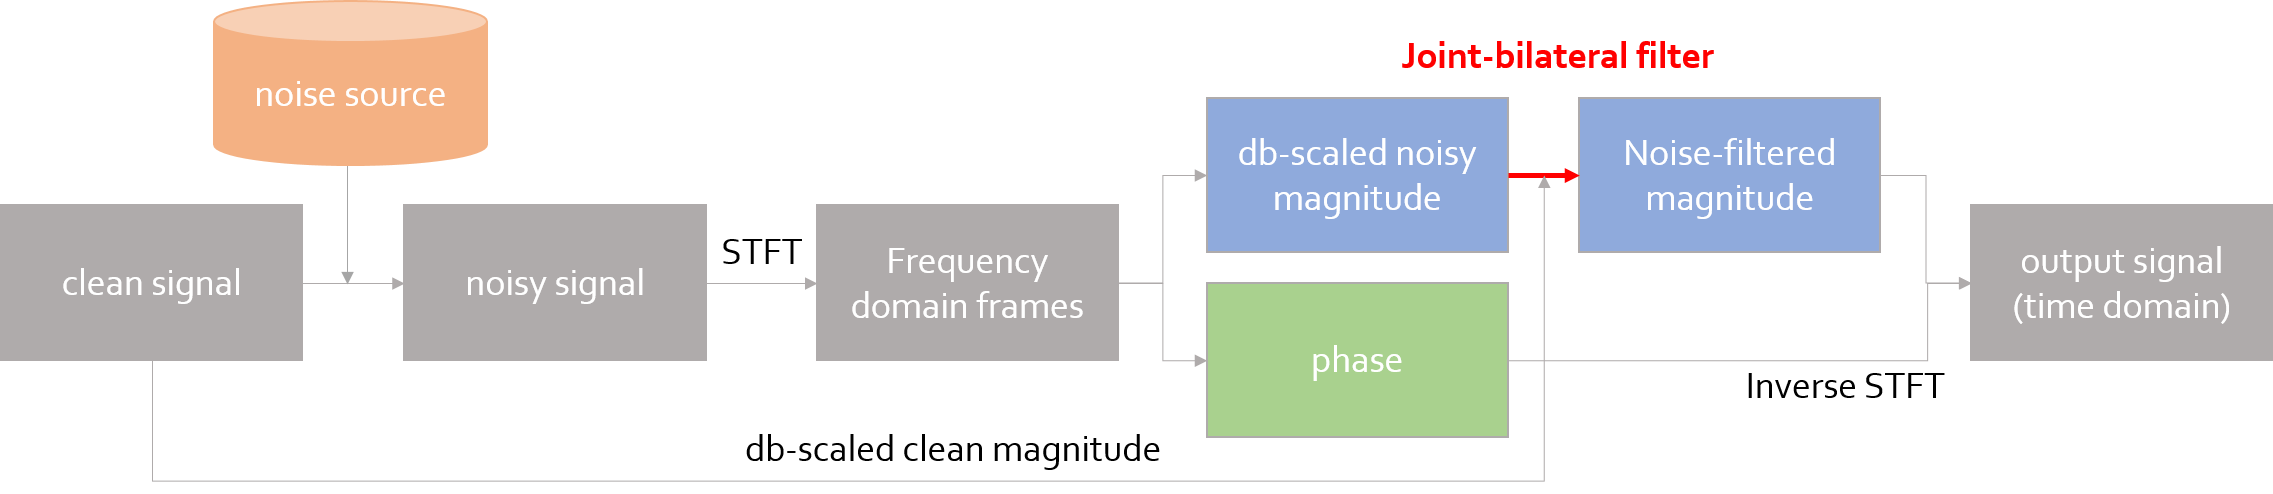
\includegraphics[width=\linewidth]{jbfilter_process}
   \caption{augmentation process using joint-bilateral filter. noised signal is filtered in 
   magnitude-frequency domain for denoising.}
   \label{fig:jbfilter_process}
\end{figure*}

Detailed process of augmenting the data, depicted in \cref{fig:jbfilter_process}, is as follows: 
First, clean speech is added with noise sources given specific Signal-to-Noise ratio (SNR).
Noise mixing is done in time domain of the signal. Next, the noisy signal is converted to complex-valued
time-frequency components by Short-Time Fourier Transform. Joint-bilateral filter is applied on log-scaled
magnitude of the frequency component after separating the complex value into magnitude and phase.
Noise-filtered log-scale magnitude and the phase are then used to reconstruct time-domain signal. 

\begin{figure}[h]
   \centering
   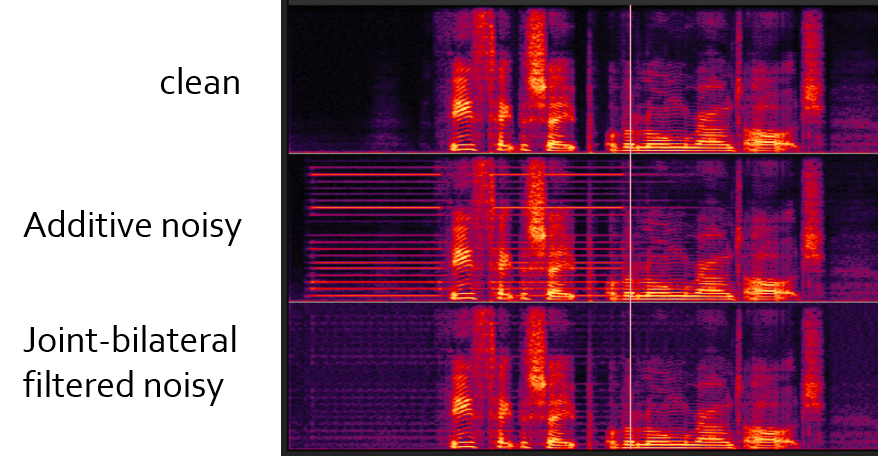
\includegraphics[width=0.9\linewidth]{jbfilter_result_v2}
   \caption{results of denoising noisy speech with joint-bilateral filter.}
   \label{fig:jbfilter_result}
\end{figure}

\cref{fig:jbfilter_result} shows spectral results of denoising noisy input with joint-bilateral filter on 
magnitude-frequency domain. Striped patterns shown along the whole frequency bins in noisy speech are 
largely suppressed after the denoising. 

\subsection{notch filter on spectro-temporal modulation}
\label{sec:notch}
Modulation spectrum~\cite{marchand2014modulation} is the evolution over time of the amplitude content 
of the various frequency bands $\omega$ of an STFT by a second Fourier Transform.
From the definition of an STFT as $x(\omega, \tau)$, modulation spectrum $X(\omega, \Omega)$ is defined
as follows: 
\begin{equation}
x(\omega, \tau) = \frac{1}{\sqrt{2\pi}}\int_t x(t)h(\tau - t)e^{-j\omega t}dt
\end{equation}
\begin{equation}
X(\omega, \Omega) = \frac{1}{\sqrt{2\pi}}\int_{\tau} |x(\omega, \tau)|e^{-j\Omega\tau}d\tau
\end{equation}
where $\omega$ is the frequencies of the STFT, $\tau$ is the center-time of the STFT windows and 
$\Omega$ is the frequencies of the second Fourier Transform. 

Spectro-temporal modulation~(\cite{chi1999spectro}, ~\cite{singh2003modulation}), also known as 
Modulation Power Spectrum (MPS), is the two-dimensional Fourier transform of the spectrogram which 
quantifies the power in temporal and spectral modulations. When regarding spectrogram as an image,
MPS can be viewed as an output of Fourier transform of the image. From the idea of a notch filter from
image domain, masking MPS on both temporal, spectral axis can help augmenting the signal.

Effect of masking speech in MPS domain can be found in \cref{fig:mps_result}. After applying 2-dimensional
Fourier transform on the magnitude of the spectrogram, masking is done on either horizontal or vertical line 
with fixed thickness. Masked MPS is then inverse-transformed to attain new magnitude spectrogram. With the 
phase information on the clean spectrogram, final output of time-domain audio signal is generated.
It can be seen in \cref{fig:mps_result} that each of masking generates different periodic artifacts 
on the output spectrogram.

\begin{figure}[h]
   \centering
   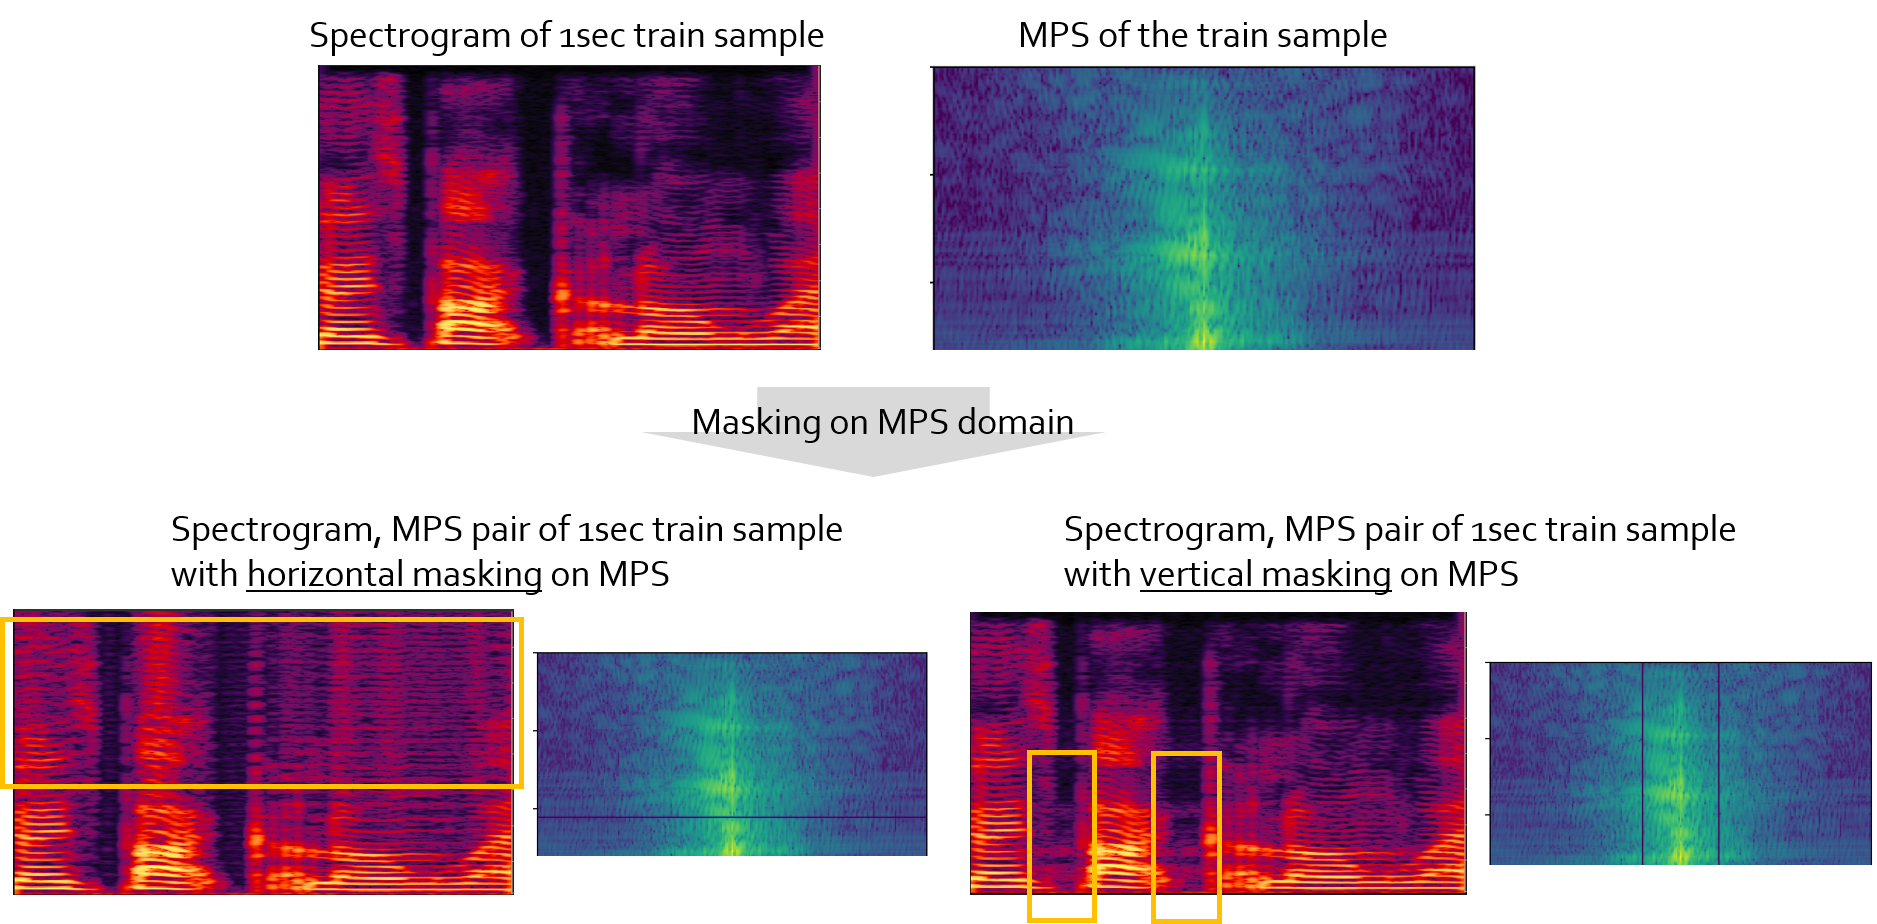
\includegraphics[width=\linewidth]{mps_result}
   \caption{result of masking on MPS domain and convert into spectrogram. Noisy artifacts having 
   periodicity on either time axis or frequency axis is added by the MPS masking.}
   \label{fig:mps_result}
\end{figure}

\subsection{popular image augmentation techniques on spectrogram}
\label{sec:popular}

Mixup~\cite{zhang2017mixup} is a commonly used image augmentation scheme which adds several images 
pixel-wise and set its label as the smoothed version of the selected classes. It is proven in several image 
classification tasks that this simple idea of populating corpus improves performance with minimal 
implementational cost. 
One variation of ~\cite{zhang2017mixup} is CutMix~\cite{yun2019cutmix} in which blockwise replacement of an image
occurs, instead of pixel-wise mixing. It also outperformed the baseline model in both ImageNet and CIFAR tasks.
In ~\cite{zhang2017mixup} simple speech augmentation result is also shown. In the experiment, the model is trained 
to classify a few of short voice commands including \textit{yes, no, down} and mixing is done on 
padded spectrogram of the signals.
In this paper, more sophisticated yet practical task is on target. Furthermore, several implementational variances 
in signal mixup schemes are compared, and analyzed.

\begin{figure}[h]
   \centering
   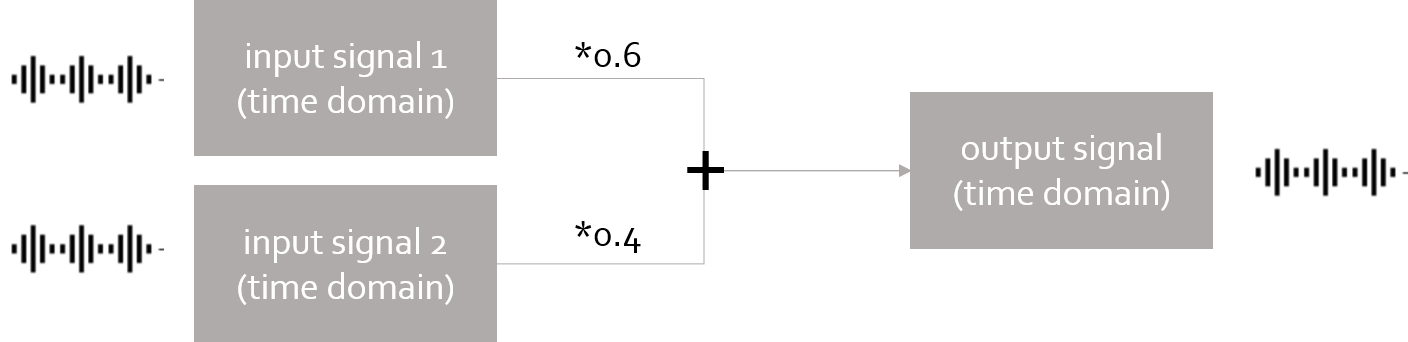
\includegraphics[width=\linewidth]{time_add}
   \caption{mixup of two speeches in time domain.}
   \label{fig:time_add}
\end{figure} 

\begin{figure}[h]
   \centering
   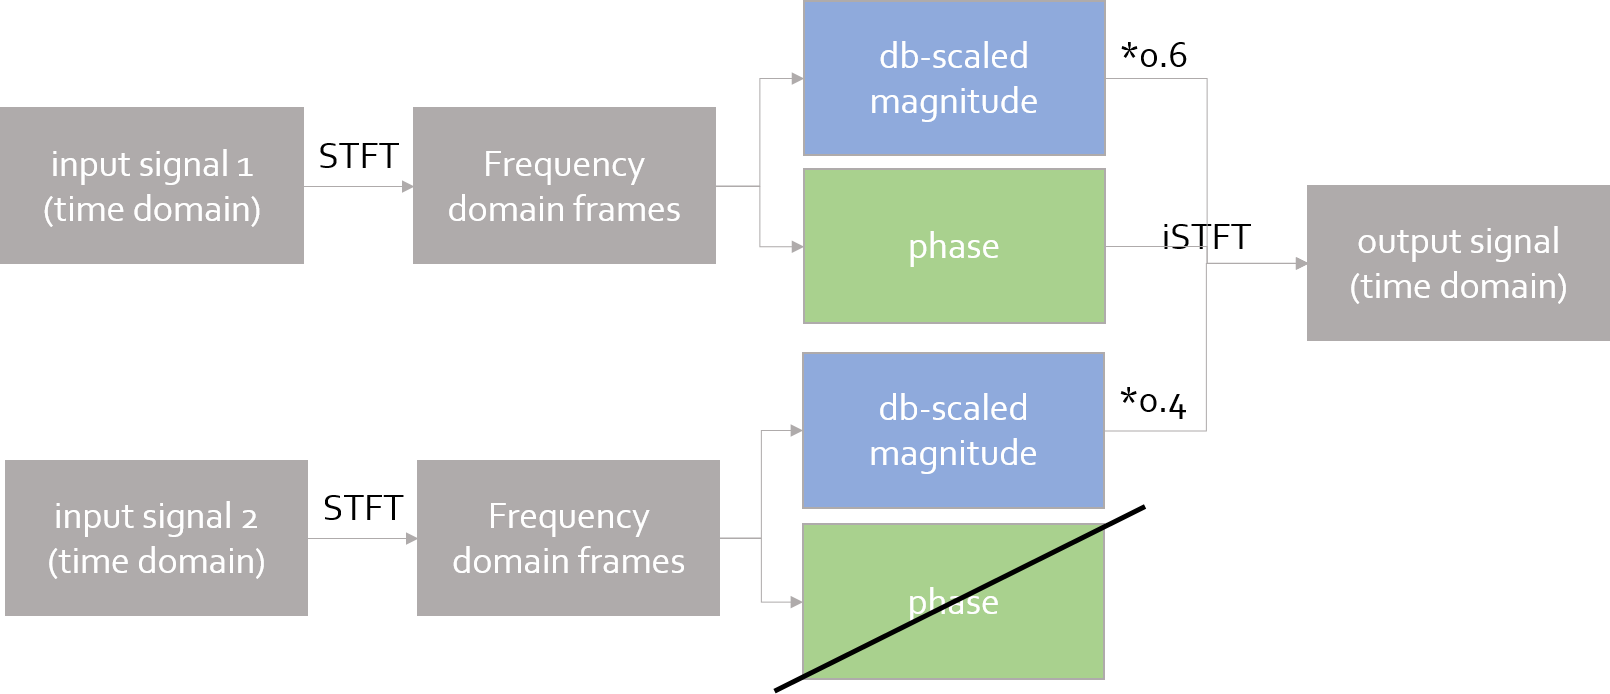
\includegraphics[width=\linewidth]{freq_add}
   \caption{mixup of two speeches in magnitude-frequency domain.}
   \label{fig:freq_add}
\end{figure} 

One of the options in mixing speeches is to add two (or more) speeches in time domain, with each of the weights.
Next option is to add magnitude-frequency of the speeches while preserving consistency on phase information;
whilst applying weighted-sum on magnitude-frequency domain, phase of a speech having the largest weight is used 
for reconstruction of the output. It enables more conservative mixing than time domain sample-wise mixing.
\cref{fig:time_add} and \cref{fig:freq_add} shows the process of the two mixing schemes.
It can be found from \cref{fig:add_result} that mixup in magnitude-frequency domain preserves most of the 
low-band component from Speech 1.

\begin{figure}[h]
   \centering
   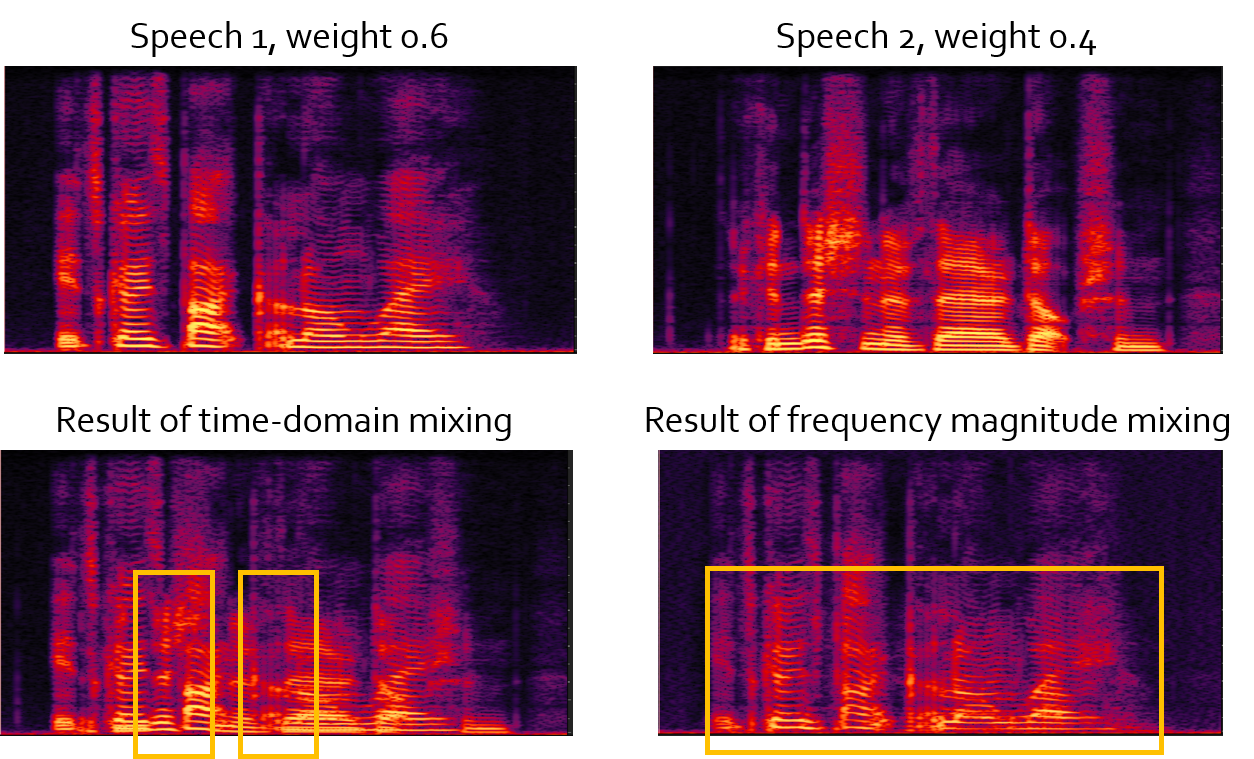
\includegraphics[width=\linewidth]{add_result}
   \caption{result after mixup in both time domain and magnitude-frequency domain.}
   \label{fig:add_result}
\end{figure}

\section{Experiments}
\label{sec:experiments}

\subsection{spatial filter on spectrogram}
To see the effectiveness of spatially-denoised corpus, speaker identification task is used as the target.
In speaker identification, the model is trained to classify the speaker id given the speech signal,
assume that every speaker in test set is contained in training set.

Training and evaluation are done on 100 speakers of VCTK~\cite{veaux2017cstr} corpus, so that
the model classifies given signal to one of 100 speaker ids.
For training, total 1.4 hours of the data is used and 30 minutes of the data is used for evaluation.
Noise augmentation on clean testset is done to test noise robustness of the model.
Noise sources for augmentation are from DEMAND~\cite{thiemann2013diverse} and MUSAN~\cite{snyder2015musan}.
There exists several types of noises in the noise sources, including music, station, traffic, etc.
As the baseline, simple Time-delayed neural network (TDNN) of size about 178KB is used. 

Evaluation results can be found in \cref{tab:spatial}. It can be seen that mixing clean corpus with 
additive noise augmented corpus makes the model robust to the noisy testset while the performance degrades on the clean testset.
The tradeoff between the noise robustness and the performace on clean testset can be controlled by the 
SNRs on noise augmentation; as the SNR gets higher, the accuracy on clean testset increases while the noise robustness decreases.
Using joint-bilateral noisy data does not harm the clean testset performance while handling the noisy testset.

\begin{table*}
   \centering
   \begin{tabular}{@{}lcr@{}lcr@{}}
     \toprule
     Training corpus & \makecell{Accuracy on \\ clean testset} & \makecell{Accuracy on \\ noisy(10db) testset} \\
     \midrule
     Clean & 89.0\% & \textcolor{red}{24.0\%} \\
     Clean + additive(10db) & \textcolor{red}{84.0\%} & 61.6\% \\
     Clean + additive(20db) & 85.2\% & 49.0\% \\
     Clean + additive(30db) & 88.8\% & 38.0\% \\
     Clean + joint-bilateral & \textbf{89.4\%} & 54.4\% \\
     Clean + additive(10db) + joint-bilateral & 85.6\% & \textbf{61.8\%} \\
     \bottomrule
   \end{tabular}
   \caption{Results on several types of training corpus.}
   \label{tab:spatial}
\end{table*}

\subsection{notch filter on spectro-temporal modulation}
Instead of speaker identification which is more suitable for checking noise-robustness of the model,
speaker verification task is used to test the feasibility of notch filtering on MPS domain.
Speaker verification model classifies whether an audio sample belongs to a predetermined person or not,
thus evaluation can be done with speech of unseen speaker.
For performance evaluation, Both Equal error rate(EER) and its threshold value are used. 
EER is the crosspoint where False acceptance rate equals False rejection rate, so lower EER 
stands for better overall verification performance.

For training and evaluation, 100 speakers on VCTK are splited by 80, 20 speakers respectively.
Total 40 hours of speech data is used in training and 6 hours are used for evaluation.
No external noise augmentation is used in the task.
X-vector~\cite{snyder2018x} of size 2.8MB is used as the base model.

\begin{table}
   \centering
   \begin{tabular}{@{}lcr@{}lcr@{}}
     \toprule
     Training corpus & \makecell{EER on testset} & \makecell{Threshold for the \\ EER (range: 0-1)} \\
     \midrule
     Clean & \textbf{1.94719\%} & 0.784438 \\
     \makecell[l]{Clean + MPS0} & 2.44224\% & 0.789325 \\
     \makecell[l]{Clean + MPS1} & 2.11221\% & 0.788875 \\
     \makecell[l]{Clean + MPS0 + MPS1} & 2.0462\% & \textbf{0.805046} \\
     \bottomrule
   \end{tabular}
   \caption{Results on several types of MPS augmentations. Thresholds along with the EER scores are reported.}
   \label{tab:notch}
\end{table}

Evaluation results can be found in \cref{tab:notch}, where MPS0 refers “masking on axis 0 of the MPS” and 
MPS1 refers “masking on axis 1 of the MPS”.
It is shown that adding MPS augmented speech degrades performance and applying MPS on axis 1 results better performance than on axis 0.
However, it can be seen that the threshold on the EER point got increased, implying the fact that 
the model gets more robust to false-acceptance.

\subsection{popular image augmentation techniques on spectrogram}
As the above section, speaker verification task is used to prove the effectiveness of the augmentation schemes.
Training, evaluation set are identical as before.
X-vector of size around 178KB is first used to test various combinations of corpora, then combination recipes 
included in top-3 performances are further trained on bigger model of size 2.8MB.

\begin{table*}
   \centering
   \begin{tabular}{@{}lcr@{}lcr@{}}
     \toprule
     Training corpus & \makecell{Model size 178KB} & \makecell{Model size 2.8MB} \\
     \midrule
     Clean & \textbf{2.34323\%} & 1.94719\% \\
     Clean(2) + Mix2(1) & 2.64026\% & - \\
     Clean(2) + MixMag2(1) & 2.50825\% & 1.91419\% \\
     Clean(2) + MixCut2(1) & 3.49835\% & - \\
     Clean(4) + MixMag2(2) + MixMag4(1) & 2.54125\% & - \\
     Clean(9) + MixMag2(3) + MixMag4(1) & 2.47525\% & \textbf{1.81518\%} \\
     \bottomrule
   \end{tabular}
   \caption{Results on several types of mixup, CutMix combinations.}
   \label{tab:popular}
\end{table*}

Evaluation results can be found in \cref{tab:popular}. In the table, Mix2 means “mixing two different time-domain signals”, 
while MixMag2 refers “mixing two different frequency magnitude signals” and MixCut2 refers 
“mixing two different time-domain signals with cutting scheme”.
Parentheses in a combination such as "Clean(2) + Mix2(1)" refers probabilities of sampling training batch from each corpus type.

It can be seen that EER on big model gets improved when adding augmented corpus.
Model trained with clean corpus gets best EER on small model, but tends to overfit on bigger size.
With additional augmentation, overfitting is alleviated on the big model.

\section{Conclusions}
\label{sec:conclusions}
In this paper, spatial filtering, frequency-domain augmentation(MPS) and mixup augmentation techniques are covered.
It could be seen in spatial filtering experiments that noise suppressed corpus tends to maintain the accuracy on clean testset 
while helping model deal with noisy testset. Further different noise suppression techniques can be further checked 
besides of the joint-bilateral filter.

Results on MPS augmentation showed degradation of the performance, while the model becomes more robust to false-acceptance.
Experiments on different masking scheme, with fine-tuned parameters on masking can be further investigated to improve the overall performance.
ALso, false-acceptance resistance can be another main topic of the augmentation scheme depending on the application of the model.
Finally, it is shown that common image augmentation techniques can improve the performance of speech processing applications.
For future work additional image augmentation schemes proven to be useful in image domain can be applied to the speech domain.

%%%%%%%%% REFERENCES
{\small
\bibliographystyle{ieee_fullname}
\bibliography{egbib}
}

\end{document}
